\subsection{Checking a card}
\begin{figure}[htp]
\begin{center}
  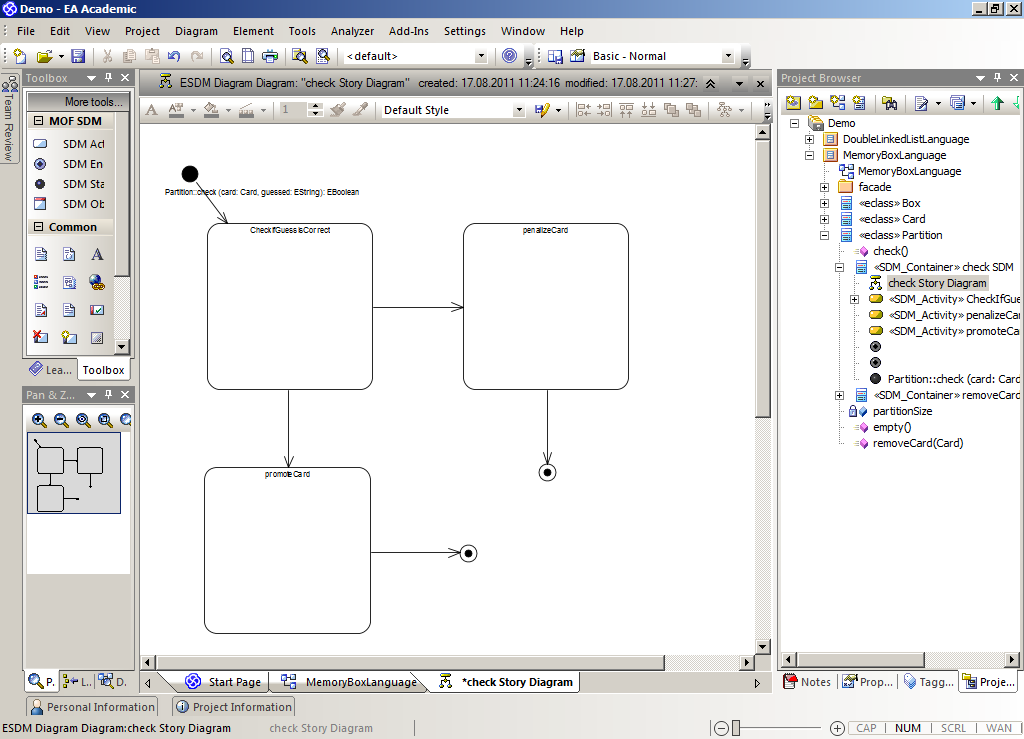
\includegraphics[width=0.7\textwidth]{pics/sdmBilder/check/sdm16RAW}
  \caption{Activity diagram for \texttt{Partition::check}.}  
  \label{fig:sdm_check_start}
\end{center}
\end{figure}

\begin{figure}[htp]
\begin{center}
  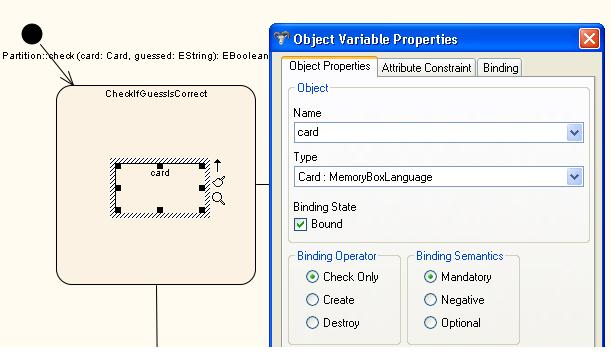
\includegraphics[width=0.7\textwidth]{pics/sdmBilder/check/sdm17RAW}
  \caption{Add the card to be checked.}  
  \label{fig:sdm_check_addCard}
\end{center}
\end{figure}

\begin{figure}[htp]
\begin{center}
  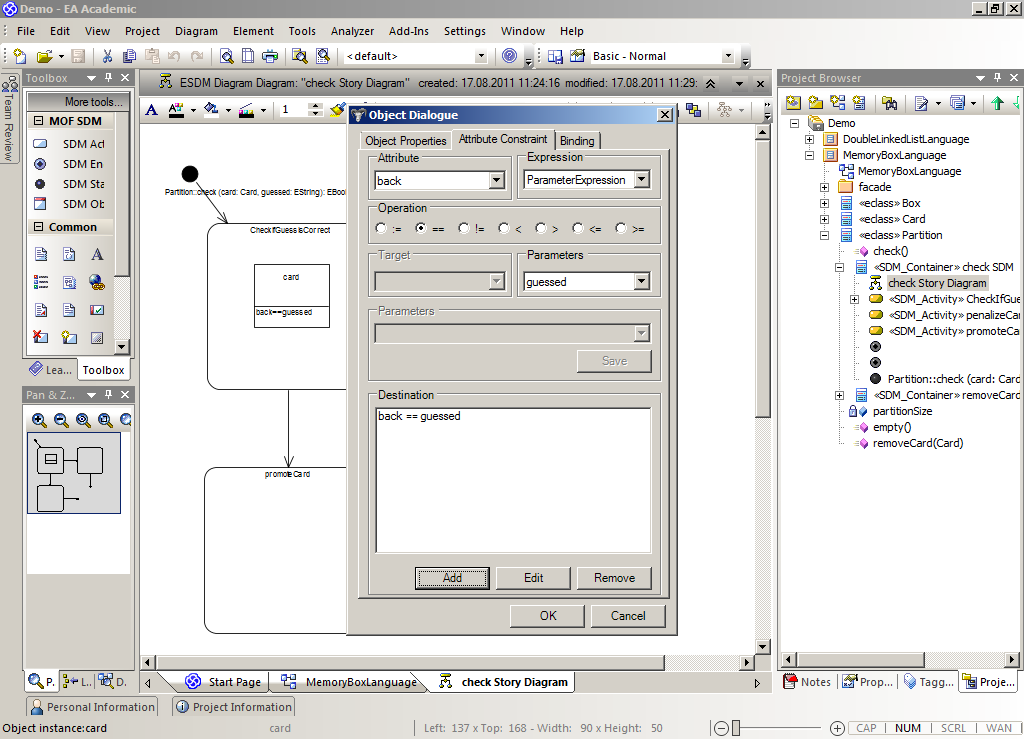
\includegraphics[width=0.7\textwidth]{pics/sdmBilder/check/sdm18RAW}
  \caption{Add an attribute constraint with a parameter expression.}  
  \label{fig:sdm_check_att_constraint}
\end{center}
\end{figure} 

\begin{figure}[htp]
\begin{center}
  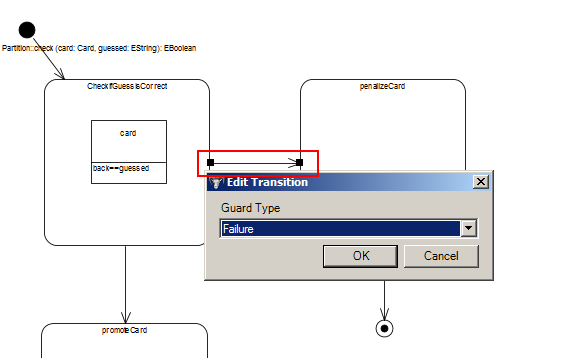
\includegraphics[width=0.7\textwidth]{pics/sdmBilder/check/sdm19}
  \caption{Add a transition with a guard.}  
  \label{fig:sdm_check_guard}
\end{center}
\end{figure}

\begin{figure}[htp]
\begin{center}
  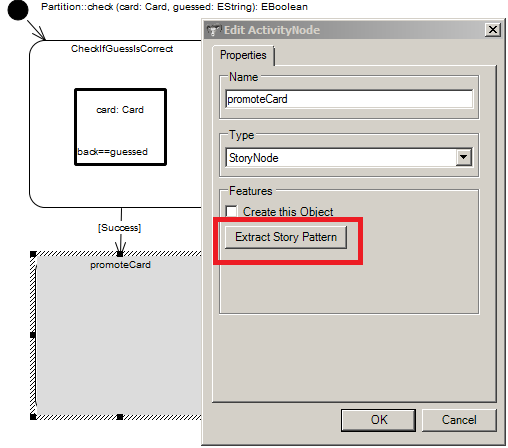
\includegraphics[width=0.7\textwidth]{pics/sdmBilder/check/sdm21}
  \caption{Extract a story pattern for more space and a better overview.}  
  \label{fig:sdm_check_extract_storypattern}
\end{center}
\end{figure}

\begin{figure}[htp]
\begin{center}
  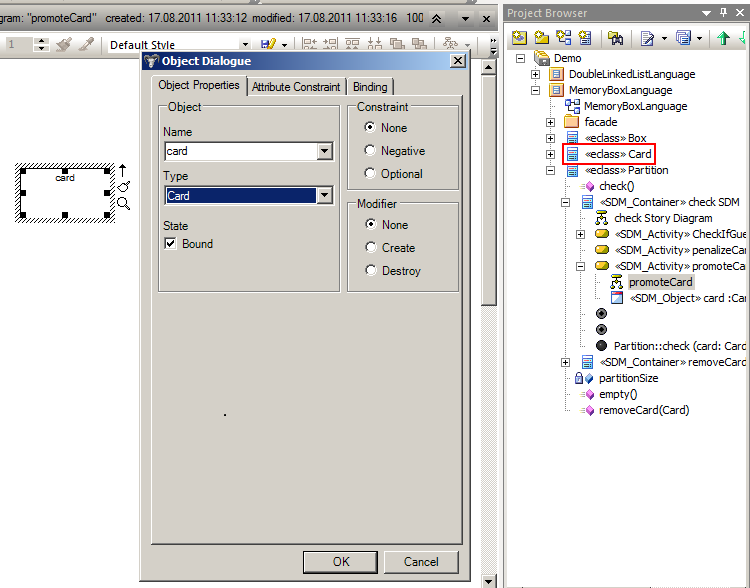
\includegraphics[width=0.7\textwidth]{pics/sdmBilder/check/sdm22RAW}
  \caption{Add an object variable \emph{bound} to a previous value.}  
  \label{fig:sdm_check_bound_card}
\end{center}
\end{figure}

\begin{figure}[htp]
\begin{center}
  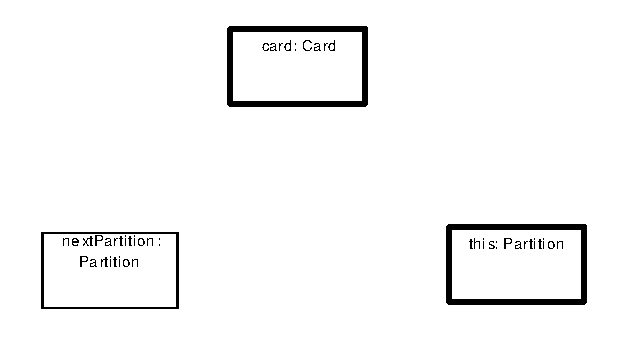
\includegraphics[width=0.7\textwidth]{pics/sdmBilder/check/sdm25}
  \caption{All object variables for story pattern.}  
  \label{fig:sdm_check_complete_sp}
\end{center}
\end{figure}

\begin{figure}[htp]
\begin{center}
  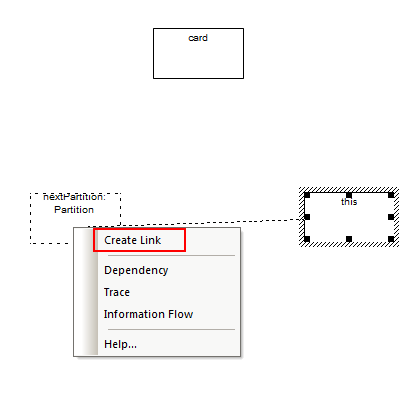
\includegraphics[width=0.7\textwidth]{pics/sdmBilder/check/sdm26}
  \caption{Create a link variable.}  
  \label{fig:sdm_check_link_variable}
\end{center}
\end{figure}

\begin{figure}[htp]
\begin{center}
  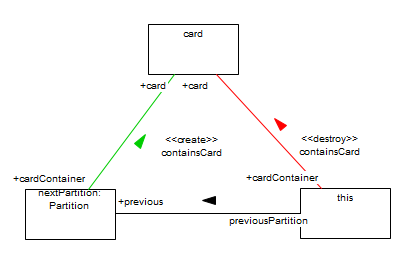
\includegraphics[width=0.7\textwidth]{pics/sdmBilder/check/sdm30}
  \caption{Complete story pattern for activity node \texttt{promoteCard}.}  
  \label{fig:sdm_check_complete_activity_node}
\end{center}
\end{figure}

\begin{figure}[htp]
\begin{center}
  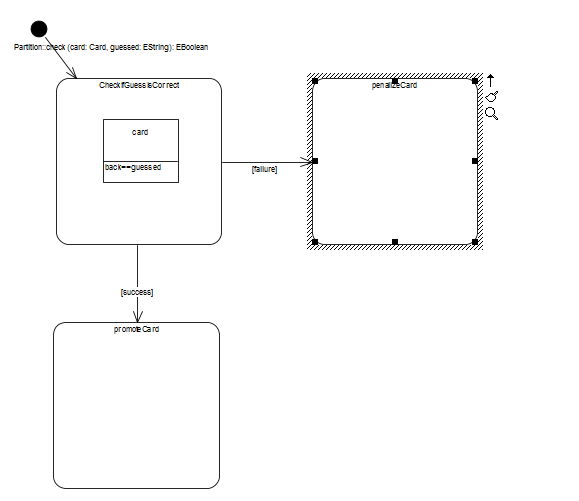
\includegraphics[width=0.7\textwidth]{pics/sdmBilder/check/sdm31}
  \caption{Extract story pattern for activity node \texttt{penalizeCard}.}  
  \label{fig:sdm_check_start_penalize}
\end{center}
\end{figure}

\begin{figure}[htp]
\begin{center}
  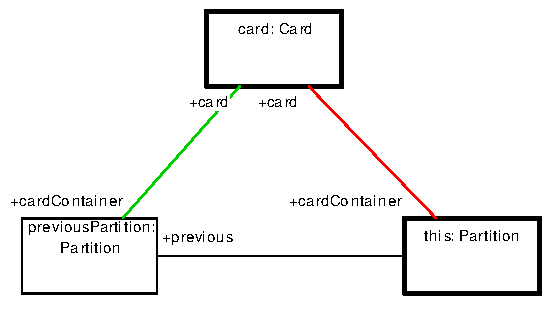
\includegraphics[width=0.7\textwidth]{pics/sdmBilder/check/sdm38}
  \caption{Story pattern for activity node \texttt{penalizeCard}.}  
  \label{fig:sdm_check_complete_penalize}
\end{center}
\end{figure}

\begin{figure}[htp]
\begin{center}
  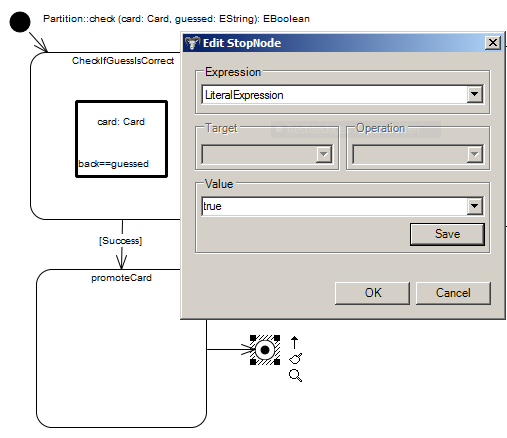
\includegraphics[width=0.7\textwidth]{pics/sdmBilder/check/sdm39}
  \caption{Add a return value with a literal expression.}  
  \label{fig:sdm_check_literal_exp}
\end{center}
\end{figure}

\begin{figure}[htp]
\begin{center}
  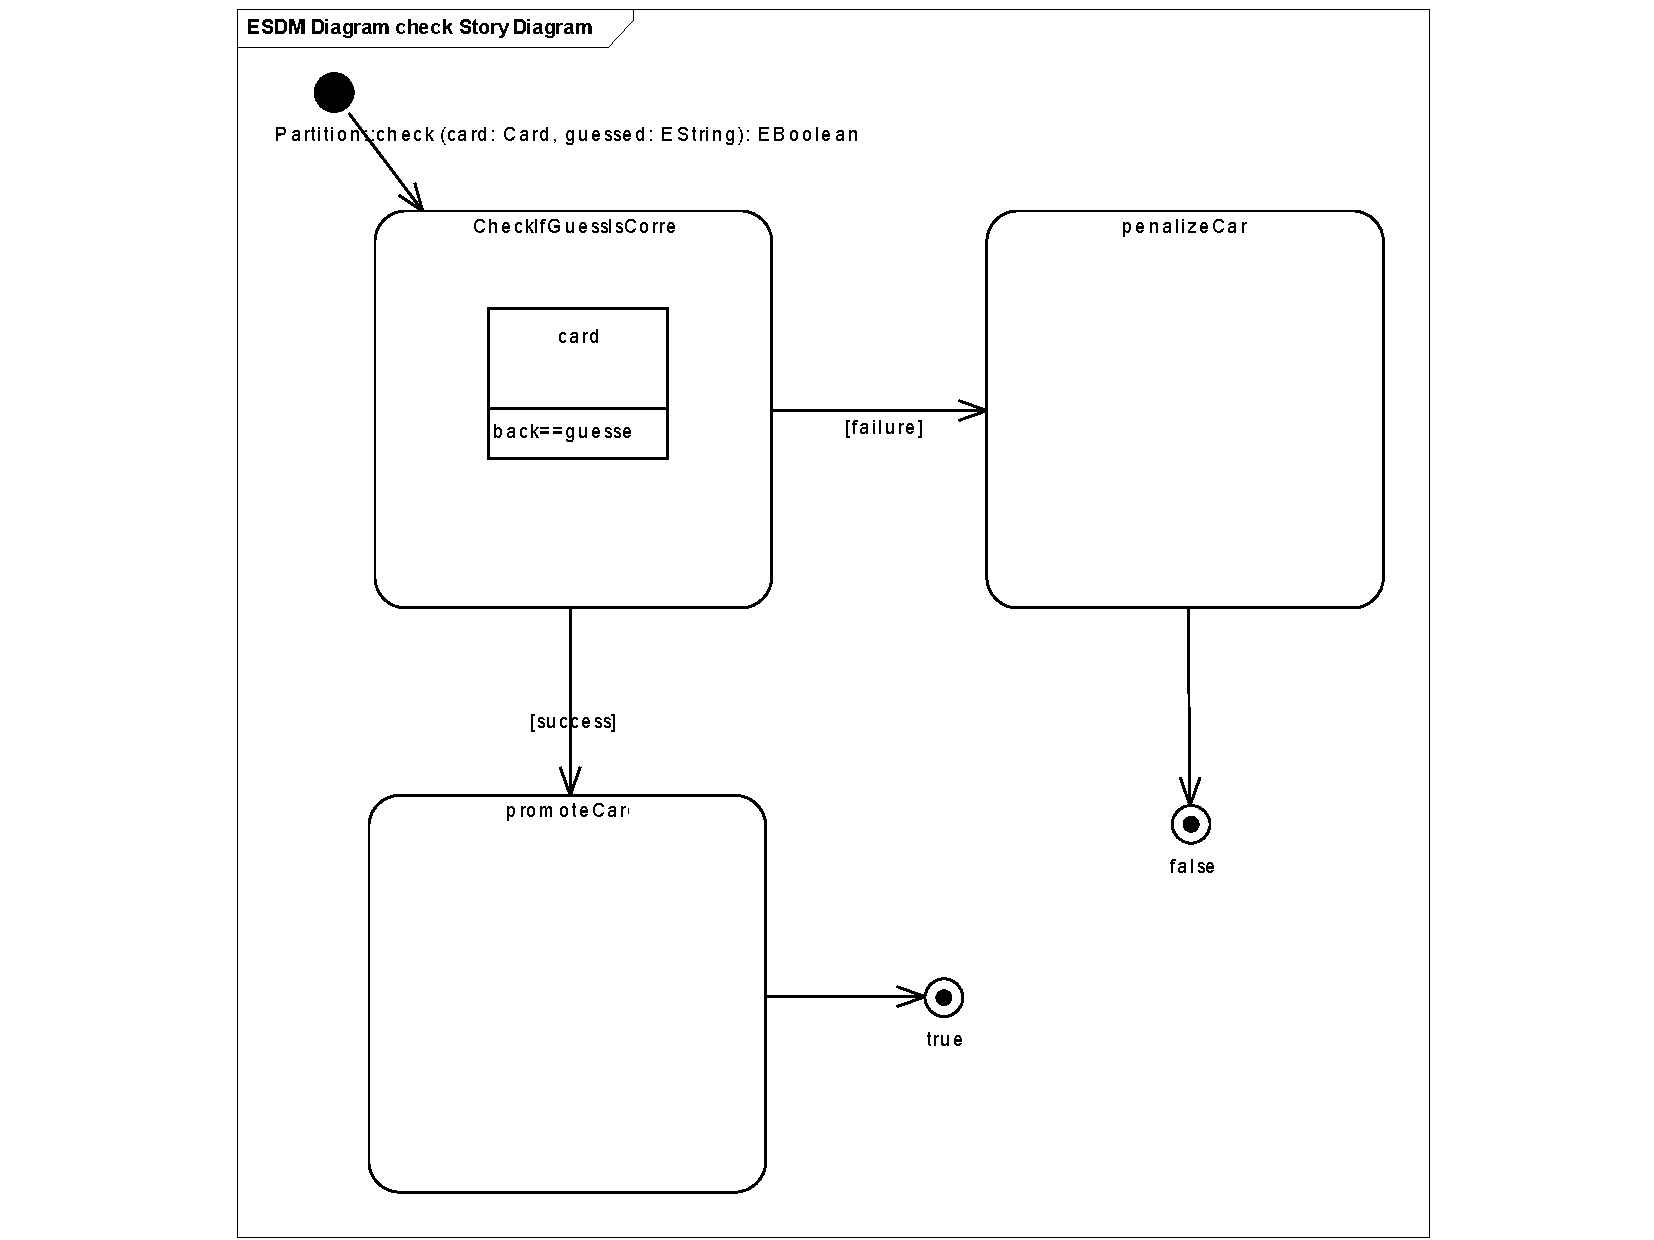
\includegraphics[width=0.7\textwidth]{pics/sdmBilder/check/sdm40}
  \caption{Complete SDM for \texttt{Partition::check}.}  
  \label{fig:sdm_check_finish}
\end{center}
\end{figure}

\clearpage 